\documentclass{article}
	
\usepackage[margin=1in]{geometry}		% For setting margins
\usepackage{amsmath}				% For Math
\usepackage[]{amssymb}
\usepackage{amsmath}
\usepackage{gensymb}
\usepackage{fancyhdr}				% For fancy header/footer
\usepackage{graphicx}				% For including figure/image
\usepackage{cancel}					% To use the slash to cancel out stuff in work
\usepackage{wasysym}                % For cent symbol
\usepackage{needspace}              % To force item to next page

%%%%%%%%%%%%%%%%%%%%%%
% Set up fancy header/footer
\pagestyle{fancy}
\fancyhead[RO,R]{{\large\textbf{PHYS-102}}}
\fancyhead[LO,L]{\large{\textbf{Ch 13 Problem Set}}}
% \fancyhead[CO,C]{\large{\textbf{Part 1}}}
% \fancyhead[RO,R]{\today}
\fancyfoot[LO,L]{}
\fancyfoot[CO,C]{\thepage}
\fancyfoot[RO,R]{}
\renewcommand{\headrulewidth}{0.4pt}
\renewcommand{\footrulewidth}{0.4pt}
%%%%%%%%%%%%%%%%%%%%%%

\newcommand{\hmwkTitle}{Chapter 13 Fluids}
% \newcommand{\hmwkDueDate}{February 12, 2014}
\newcommand{\hmwkClass}{PHYS-102}
% \newcommand{\hmwkClassTime}{}
% \newcommand{\hmwkClassInstructor}{Professor Isaac Newton}
\newcommand{\hmwkAuthorName}{\textbf{\underline{\hspace{3in}}}}

% math shortcuts
\newcommand\rr{\quad\Rightarrow\quad}

%
% Title Page
%

\title{
    \vspace{2in}
    \textmd{\textbf{\hmwkTitle}}\\
    \vspace{0.5in}
    \textmd{\textbf{\hmwkClass}}\\
    % \normalsize\vspace{0.1in}\small{Due\ on\ \hmwkDueDate\ at 3:10pm}\\
    % \vspace{0.1in}\large{\textit{\hmwkClassInstructor\ \hmwkClassTime}}
    \vspace{4in}
}

\author{\hmwkAuthorName}
\date{}
\begin{document}
\maketitle
\newpage
\begin{center}
    \section*{\textbf{\underline {Conceptual Questions}}}
\end{center}
\subsubsection*{
    1. If one material has a higher density than another, must the molecules
    of the first be heavier than those of the second? Explain.
}
No. If one material has a higher density, it can either be that, yes, it's
heavier, but it could also be because they are packed closer together (less
volume). Symbolic relationship of mass, density, and volume: \rho =
\displaystyle\frac{m}{V}
\subsubsection*{
    8. Will an ice cube float in a glass of alcohol? Why or why not? 
}
Alcohol is less dense than water so no. In order to float, the ice cube would
have to displace a weight of alcohol = to its own weight; however, given that
alcohol is less dense, this is impossible.
\subsubsection*{
    9. A submerged can of Coke® will sink, but a can of Diet
    Coke® will float. (Try it!) Explain.
}
As a baseline, all carbonated drinks hace a gas dissolved in them so their
desnity is less than water causing them to float. However, normal Coke also has
a bunch of sugar dissolved in it which increases density causing it to sink. On
the other hand, Diet Coke has no sugar which, with only the gas dissolved in it,
will float.
\subsubsection*{
    13. Explain why helium weather balloons, which are used to measure 
    atmospheric conditions at high altitudes, are normally released while 
    filled to only 10–20\% of their maximum volume.
}
As the weather balloon rises into the upper atmosphere, atmospheric pressure on
it decreases, allowing the balloon to expand as the gas inside it expands. If
filled to max, the balloon would burst shortly after take-off.
\subsubsection*{
    17. If you dangle two pieces of paper vertically, a few inches apart 
    (Fig. 13–45), and blow between them, how do you think the papers will
    move? Try it and see. Explain.
}
\begin{figure}[h]
    \begin{center}
        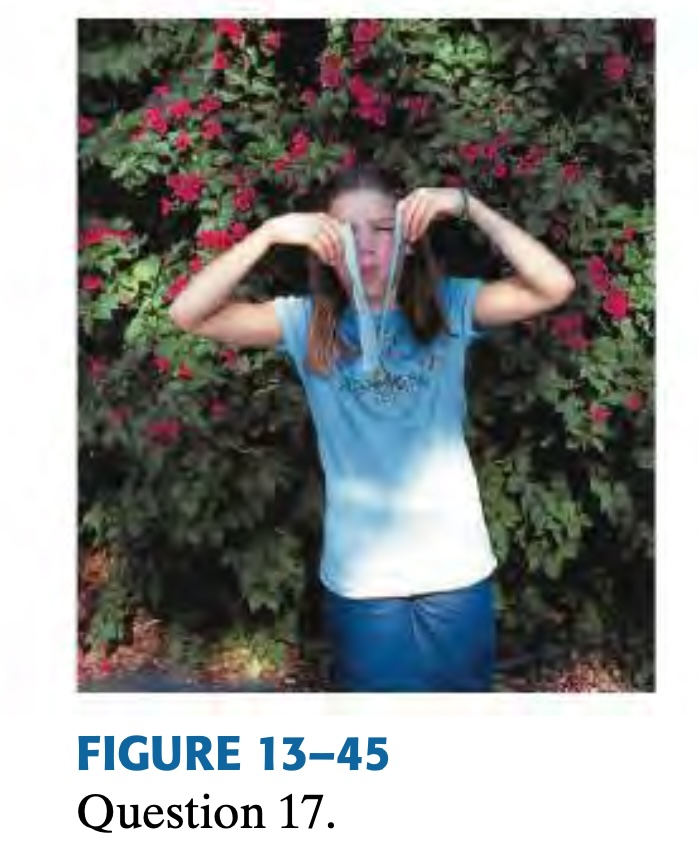
\includegraphics[width=0.3\textwidth]{figures/17.jpg}
    \end{center}
\end{figure}
The papers will move toward each other. When you blow between the sheets of
paper, you reduce the air pressure between them (Bernoulli's principle). The
greater air pressure on the other side of each sheet will push the sheets toward
each other. 
\subsubsection*{
    18. Why does the stream of water from a faucet become narrower as it
    falls (Fig. 13–46)?
}
\begin{figure}[h]
    \begin{center}
        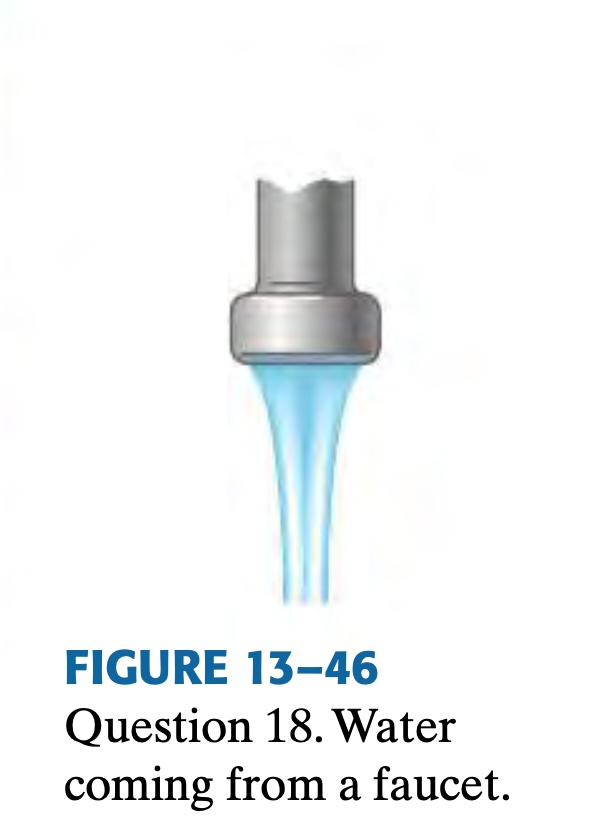
\includegraphics[width=0.3\textwidth]{figures/18.jpg}
    \end{center}
\end{figure}
As the water falls, it speeds up due to gravity. Because the volume flow rate
($Q = A\vec v$) must remain constant, the faster moving water's cross-sectional
area must be smaller. 
\subsubsection*{
    19. Children are told to avoid standing too close to a rapidly moving
    train because they might get sucked under it. Is this possible? Explain.
}
As the train travels, it pulls some air towards it Combine this with the lower
air pressure around it because of its large velocity creating a force pulling
toward the train from "high-pressure outer" to "low-pressure inner",
$\therefore$ yes it can.
\subsubsection*{
    21. Why do airplanes normally take off into the wind?
}
Taking off into the wind increases the velocity of the plane relative to the
air, an important factor in the creation of lift. The plane will be able to take
off with a slower ground speed, and a shorter runway distance
\subsubsection*{
    23. Why does the canvas top of a convertible bulge out when
    the car is traveling at high speed? [Hint: The windshield
    deflects air upward, pushing streamlines closer together.]
}
Due to the air moving fast outside the car, due to Bernoulli's Principle, the
air pressure in the car will be greater than that of outside the car.
$\therefore$ The air will try traveling outside the car causing the top to bulge
out.
\subsubsection*{
    24. Roofs of houses are sometimes “blown” off (or are they pushed off?)
    during a tornado or hurricane. Explain using Bernoulli’s principle.
}
Typically, the inside vs. outdoor air pressure is usually the same. However, at
the event of a tornado or hurricane, the air pressure may suddenly drop outside
causing the indoor air pressure to "push" the roof off. 
\newpage
\begin{center}
    \section*{\textbf{\underline {Problems}}}
\end{center}
\begin{center}
    \subsection*{\textbf{\textit{13-2 Density and Specific Gravity}}}
\end{center}
\subsubsection*{
    1. The approximate volume of the granite monolith known as El Capitan
    in Yosemite National Park (Fig. 13–47) is about $10^8$ $m^3$. 
    What is its approximate mass?
}
\begin{figure}[h]
    \begin{center}
        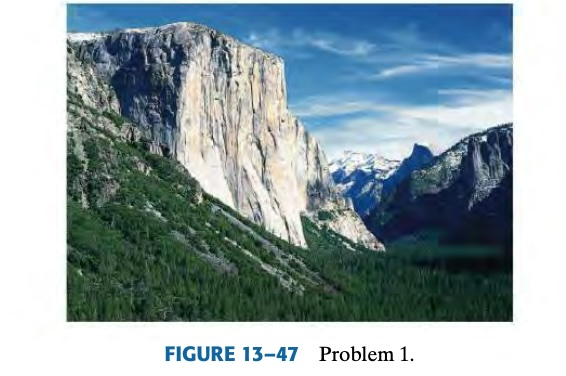
\includegraphics[width=0.5\textwidth]{figures/p1.jpg}
    \end{center}
\end{figure}
\begin{align*}
    \intertext{The density of grantite is $\rho = 2.7 \times 10^3 \frac{kg}{m^3}$}
    m &= \rho V \\
    m &= (2.7 \times 10^3 \frac{kg}{m^3})(10^8 m^3) \\
    m &\approx 2.7 \times 10^{11} kg
\end{align*}
\subsubsection*{
    2.  What is the approximate mass of air in a living room $5.6m \times 3.8m \times 2.8m$?
}
\begin{align*}
    V &= (5.6m)(3.8m)(2.8m) \\
    V &= 59.584 m^3 \approx 60 m^3 \\\\
    \rho_{air} &= 1.29 \displaystyle\frac{kg}{m^3}\\\\
    \therefore m &= \rho V = (1.29 \displaystyle\frac{kg}{m^3})(60 m^3) \\
    m &\approx 77\;kg
\end{align*}
\subsubsection*{
    3. If you tried to smuggle gold bricks by filling your backpack, whose dimensions
    are $56 cm \times 28 cm \times 22 cm$, what would its mass be?
}
\begin{align*}
    \intertext{The density of gold is $\rho_{gold} = 19.3 \times 10^3
    \displaystyle\frac{kg}{m^3}$}
    V &= (0.56 m)(0.28 m)(0.22 m) \\
    V &\approx 0.034 m^3 \;or\; 3.4 \times 10^{-2} m^3 \\\\
    \therefore m &= \rho V = (19.3 \times 10^3 \displaystyle\frac{kg}{m^3})(3.4
    \times 10^-2 m^3) \\
    m &\approx 670\;kg
\end{align*}
\newpage
\begin{center}
    \subsection*{\textbf{\textit{13-3 to 13-6 Pressure; Pascal's Principle}}}
\end{center}
\subsubsection*{
    9. Estimate the pressure exerted on a floor by (a) one pointed chair leg
    (66 kg on all four legs) of area = 0.020 $cm^2$, and (b) a 1300-kg elephant
    standing on one foot (area = 800 $cm^2$).
}
\begin{align*}
    \intertext{a.} 
    P &= \displaystyle\frac{\text{Force}}{\text{Area}} = \displaystyle\frac{F}{A}
    \intertext{The force would be $\frac 1 4$ the weight of the chair since it
    is standing on just one leg}
    P &= \displaystyle\frac{\frac 1 4 mg}{A} \\
    P &= \displaystyle\frac{\frac 1 4 (66\;kg)(9.8
    \displaystyle\frac{m}{s^2})}{0.00020\;m^2} \\
    P &\approx 808500 \displaystyle\frac{N}{m^2}
    \intertext{b.}
    P &= \displaystyle\frac{\text{Force}}{\text{Area}} = \displaystyle\frac{F}{A} \\
    P &= \displaystyle\frac{mg}{A} \\
    P &= \displaystyle\frac{(1300\;kg)(9.8 \displaystyle\frac{m}{s^2})}{8 m^2} \\
    P &\approx 1593 \displaystyle\frac{N}{m^2}
\end{align*}
\subsubsection*{
    14. The gauge pressure in each of the four tires of an automobile is
    240 kPa. If each tire has a “footprint” of 220 $cm^2$, estimate the mass of the car.
}
\begin{align*}
    P &= \displaystyle\frac{\text{Force}}{\text{Area}} = \displaystyle\frac{F}{A} \\
    P &= \displaystyle\frac{mg}{A} \\
    m &= \displaystyle\frac{PA}{g}
    \intertext{Since each of the tires is exerting a pressure within their
    respective area, this would be $4PA$}
    m &= \displaystyle\frac{4PA}{g} = \displaystyle\frac{4(240000
    \displaystyle\frac{\displaystyle\frac{kg\cdot m}{s^2}}{m^2})(0.022 m^2)}{9.8
    \displaystyle\frac{m}{s^2}} \\
        m &= 2155\;kg \approx 2200\;kg
\end{align*}
\subsubsection*{
    18. In working out his principle, Pascal showed dramatically how force
    can be multiplied with fluid pressure. He placed a long, thin tube of radius
    r = 0.30 cm vertically into a wine barrel of radius R = 21 cm, Fig. 13–50.
    He found that when the barrel was filled with water and the tube filled to a
    height of 12 m, the barrel burst. Calculate (a) the mass of water in the tube,
    and (b) the net force exerted by the water in the barrel on the lid just before rupture.
}
\begin{figure}[h]
    \begin{center}
        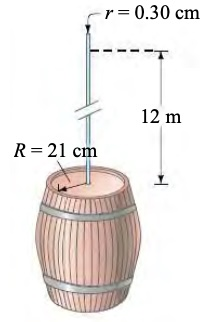
\includegraphics[width=0.2\textwidth]{figures/p18.jpg}
    \end{center}
\end{figure}
\begin{align*}
    \intertext{a. We use the definition of density and notice the shape of the
    tube is a cylinder}
    m &= \rho V = \rho (\pi r^2h) \\
    m &= (1000 \displaystyle\frac{kg}{m^3})(\pi)(0.003m)^2(12m) \\
    m &\approx 0.34\;kg
    \intertext{
        b. The net force exerted on the lid is the gauge pressure of
        the water times the area of the lid. The gauge pressure is 
        found from Eq. 13-3.
    }
    F &= PA \quad (P=\rho gh)(A = \pi r^2) \\
    F &= \rho g h \pi r^2 \\
    F &= (1000 \displaystyle\frac{kg}{m^3})(9.8
    \displaystyle\frac{m}{s^2})(12m)(\pi)(0.21m)^2 \\
    F &\approx 1.6 \times 10^4\;N
\end{align*}
\newpage
\begin{center}
    \subsection*{\textbf{\textit{13-7 Buoyancy and Archimedes' Principle}}}
\end{center}
\subsubsection*{
    27. A geologist finds that a Moon rock whose mass is 9.28 kg has an apparent
    mass of 6.18 kg when submerged in water. What is the density of the rock? 
}
\begin{align*}
    \intertext{Recall, Archimedes' Principle states that the buoyant force is
    equal to the weight of the fluid displaced}
    F_B &= \Delta \vec w  \\
    F_B &= [(9.28\;kg)(9.8 \displaystyle\frac{m}{s^2})] - [(6.18\;kg)(9.8
    \displaystyle\frac{m}{s^2})] \\
    F_B &\approx 30.38\;N
    \intertext{We can equate the buoyant force we found to the weight of the
    displaced fluid}
    F_B &= mg = \rho_{H_2O} V_{rock} g =
    \rho_{H_2O}(\displaystyle\frac{m_{rock}}{\rho_{rock}})g \\
    F_B &= \rho_{H_2O}(\displaystyle\frac{m_{rock}}{\rho_{rock}})g 
    \intertext{so, }
    \rho_{rock} &= \displaystyle\frac{\rho_{H_2O}m_{rock}g}{F_B} \\
    \rho_{rock} &= \displaystyle\frac{(1000\;\displaystyle\frac{kg}{m^3})(9.28\;kg)(9.8
    \displaystyle\frac{m}{s^2})}{30.38 \displaystyle\frac{kg\cdot m}{s^2}} \\
    \rho_{rock} &\approx 2994 \displaystyle\frac{kg}{m^3}
\end{align*}
\subsubsection*{
    35. The specific gravity of ice is 0.917, whereas that of seawater is 1.025.
    What percent of an iceberg is above the surface of the water?
}
\begin{align*}
    \intertext{The buoyant force on the ice is equal to the weight of the ice,
    since it floats.}
    F_B &= \vec w_{ice} \\
    m_{sea}g &= m_{ice}g \\
    \rho_{sea} V_{sea} &= \rho_{ice} V_{ice}
    \intertext{Let SG = Specific Gravity}
    SG_{sea}\rho_{sea}V_{sea} &= SG_{ice}\rho_{ice}V_{ice} \\
    V_{sub.\;ice} &= \displaystyle\frac{SG_{ice}}{SG_{sea}}V_{ice} \\
    V_{sub.\;} &= \displaystyle\frac{0.917}{1.025}V_{ice} \\
    V_{sub.\;ice} &\approx 0.895 V_{ice} \\
    V_{above} &= V_{ice} - V_{sub.\;ice} = 0.105 \\
    V_{above} &\approx 10.5\%
\end{align*}
\newpage
\begin{center}
    \subsection*{\textbf{\textit{13-8 to 13-10 Fluid Flow, Bernoulli's Equation}}}
\end{center}
\subsubsection*{
    45. How fast does water flow from a hole at the bottom of a very wide,
    5.3-m-deep storage tank filled with water? Ignore viscosity.
}
\begin{align*}
    \intertext{Using Torricelli's Theorem,}
    \vec v_1 &= \sqrt{2g\Delta y} \\
    \vec v_1 &= \sqrt{2(9.8 \displaystyle\frac{m}{s^2})(5.3m)} \\
    \vec v_1 &\approx 10.19 \frac m s \approx 10 \frac m s
\end{align*}
\subsubsection*{
    49. A 180-km/h wind blowing over the flat roof of a house causes the roof
    to lift off the house. If the house is $6.2 m \times 12.4m$ in size,
    estimate the weight of the roof. Assume the roof is not nailed down.
}
\begin{align*}
    \intertext{First converting the given information: $\vec v =
    (\displaystyle\frac{180km}{1h})(\displaystyle\frac{1h}{3600s})(\displaystyle\frac{1000m}{1km}) = 50 \frac m s$ and $A = 77m^2$}
    \intertext{Using Bernoulli's Equation,}
    P_{inside} + \frac 1 2 \rho\vec v_{inside}^2 + \rho gy_{inside} &=
    P_{outside} + \frac 1 2 \rho\vec v_{outside}^2 + \rho gy_{outside} \\
    \intertext{We are left with, (assuming no velocity in the house and no
    $\Delta y$.)}
    P_{in} - P_{out} &= \frac 1 2 \rho\vec v_{out}^2 \\
    \intertext{We see that $P_{in} = P_{out}$ can be rewritten as $\Delta P$}
    \intertext{Using Pascal's Principle, (net force on the roof due to air is
    the difference in pressure on the two sides of the roof $\times$ the area of
the roof)}
    \Delta P &= \displaystyle\frac{F_{air}}{A_{roof}} \\
    F_{air} &= \Delta P A_{roof} \\
    F_{air} &= \frac 1 2 \rho_{air}\vec v_{out}^2 A_{roof} \\
    F_{air} &= \frac 1 2 (1.29\frac{kg}{m^3})(50\frac m s)^2(77m^2) \\
    F_{air} &\approx 1.2 \times 10^5\;N
\end{align*}
\subsubsection*{
    52. What is the lift (in newtons) due to Bernoulli’s principle on a wing of
    area 88 $m^2$ if the air passes over the top and bottom surfaces at speeds of
    280 m/s and 150 m/s, respectively?
}
\begin{align*}
    \intertext{Using Bernoulli's Equation,}
    P_{top} + \frac 1 2 \rho\vec v_{top}^2 + \rho gy_{top} &= P_{bot} + \frac 1 2 \rho\vec v_{bot}^2 + \rho gy_{bot} \\
    P_{bot} - P_{top} &= \frac 1 2 \rho(\vec v^2_{top} - \vec v^2_{bot}) \\
    \intertext{Using Pascal's Principle,} 
    P_{bot} - P_{top} &= \displaystyle\frac{F_{lift}}{A_{wing}} \\
    F_{lift} &= \Delta PA_{wing} \\ 
    F_{lift} &= \frac 1 2 \rho (\vec v^2_{top} - \vec v^2_{bot})A_{wing} \\
    F_{lift} &= \frac 1 2 (1.29 \displaystyle\frac{kg}{m^3})\left[(280 \frac m s)^2 -
    (150 \frac m s)^2\right](88m^2) \\
    F_{lift} &\approx 3.2 \times 10^6\;N
\end{align*}
\subsubsection*{
    54. Water at a gauge pressure of 3.8 atm at street level flows into an
    office building at a speed of 0.68 m/s through a pipe 5.0 cm in diameter.
    The pipe tapers down to 2.8 cm in diameter by the top floor, 18 m above
    (Fig. 13–54), where the faucet has been left open. Calculate the flow
    velocity and the gauge pressure in the pipe on the top floor. Assume no
    branch pipes and ignore viscosity.
}
\begin{figure}[h]
    \begin{center}
        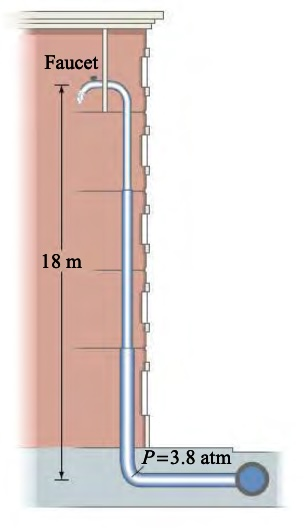
\includegraphics[width=0.2\textwidth]{figures/p54.jpg}
    \end{center}
\end{figure}
\begin{align*}
    \intertext{$A_1\vec v_1 = A_2\vec v_2$ continuity of flow rate}
    \vec v_2 &= \displaystyle\frac{A_1}{A_2}\vec v_1 \\
    \vec v_2 &= \displaystyle\frac{\pi(0.05m)^2}{\pi(0.028m)^2}(0.68\frac m s) \\
    \vec v_2 &\approx 2.17\frac m s \quad\text{flow velocity} \\
    \intertext{Using Bernoulli's Equation,}
    P_{1} + \frac 1 2 \rho_{H_2O}\vec v_{1}^2 + \rho gy_{1} &= P_{2} + \frac 1 2 \rho_{H_2O}\vec v_{2}^2 + \rho gy_{2} \\
    P_2 &= P_1 + \frac 1 2 \rho(\vec v_1^2 - \vec v_2^2) - \rho gy_2 \\
    P_2 = (3.8atm)(\displaystyle\frac{1.013\times 10^5 \frac{N}{m^2}}{1atm}) &+
\frac 1 2 (1000 \frac{kg}{m^3})\left[(0.68\frac m s)^2 - (2.17\frac m s)^2\right] - (1000 \frac{kg}{m^3})(9.8 \frac m {s^2})(-18m) \\
    P_2 &\approx 2.064\timees 10^5
    \displaystyle\frac{N}{m^2}\left(\frac{1atm}{1.013\times 10^5 \frac{N}{m^2}}\right) \\
    P_2 &\approx 2.0atm\;\text{gauge pressure}
\end{align*}
\subsubsection*{
    55. n Fig. 13–55, take into account the speed of the top surface of the
    tank and show that the speed of fluid leaving the opening at the bottom is 
    \[
        v_1 = \sqrt{\displaystyle\frac{2gh}{(1-\frac{A^2_1}{A^2_2})}}
    \]
    where $h = y_2 - y_1$, and $A_1$ and $A_2$ are the areas of the opening and
    of the top surface, respectively. Assume $A_1 << A_2$ so that the flow
    remains nearly steady and laminar 
}
\begin{figure}[h]
    \begin{center}
        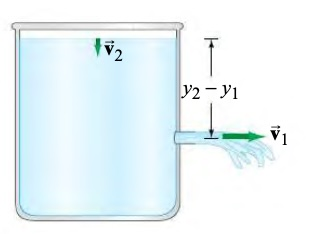
\includegraphics[width=0.3\textwidth]{figures/p55.jpg}
    \end{center}
\end{figure}
\begin{align*}
    \intertext{$A_1\vec v_1 = A_2\vec v_2$ continuity of flow rate}
    \vec v_2 &= \displaystyle\frac{A_1}{A_2}\vec v_1 \\
    \intertext{Using Bernoulli's Equation,}
    P_{1} + \frac 1 2 \rho\vec v_{1}^2 + \rho gy_{1} &= P_{2} + \frac 1 2 \rho\vec v_{2}^2 + \rho gy_{2} \\
    \intertext{$P_1 = P_2 = P_{atmosphere}$}
    \frac 1 2 \rho\vec v_1^2 - \frac 1 2 \rho\vec v_2^2 &= \rho gy_2 - \rho gy_1 \\
    \frac 1 2 \rho(\vec v_1^2 - \vec v_2^2) &= \rho g(y_2 - y_1) \\
    \vec v_1^2 - \vec v_2^2 &= 2gh \\
    \vec v_1^2 - \left(\frac{A_1}{A_2}\vec v_1\right)^2 &= 2gh \\
    \vec v_1^2 - \left(\frac{A_1^2}{A_2^2}\vec v_1^2\right) &= 2gh \\
    \vec v_1^2 \left(1 - \frac{A_1^2}{A_2^2}\right) &= 2gh \\
    \vec v_1 &= \sqrt{\displaystyle\frac{2gh}{1 - \frac{A_1^2}{A_2^2}}}
\end{align*}
\newpage
\begin{center}
    \subsection*{\textbf{\textit{General Problems}}}
\end{center}
\subsubsection*{
    97. An airplane has a mass of $1.7 \times 10^6$ kg, and the air flows
    past the lower surface of the wings at 95 m/s. If the wings have
    a surface area of 1200 $m^2$, how fast must the air flow over the
    upper surface of the wing if the plane is to stay in the air?
}
\begin{align*}
    F_{top} + mg &= F_{bot} \\
    P_{top}A + mg &= P_{bot}A \\
    (P_{bot} - P_{top}) &= \displaystyle\frac{mg}{A} \\
    \intertext{Using Bernoulli's Equation,}
    P_0 + P_{bot} + \frac 1 2 \rho\vec v_{bot}^2 + \rho gy_{bot} &= P_0 + P_{top} + \frac 1 2 \rho\vec v_{top}^2 + \rho gy_{top} \\
    P_{bot} - P_{top} + \frac 1 2 \rho\vec v_{bot}^2 &= \frac 1 2 \rho\vec
    v_{top}^2 \\
    \vec v_{top}^2 &= \displaystyle\frac{2(P_{bot} - P_{top})}{\rho} + \vec
    v_{bot}^2 \\
    \vec v_{top} &= \sqrt{\displaystyle\frac{2(P_{bot} - P_{top})}{\rho} + \vec
    v_{bot}^2} \\
    \vec v_{top} &= \sqrt{\displaystyle\frac{2mg}{\rho A}+ \vec v_{bot}^2} \\
    \vec v_{top} &= \sqrt{\displaystyle\frac{2(1.7 \times 10^6\;kg)(9.8 \frac m
    {s^2})}{(1.29 \displaystyle\frac{kg}{m^3})(1200m^2)}+ (95\frac m s)^2} \\
    \vec v_{top} &\approx 174.8 \frac m s \approx 170 \frac m s
\end{align*}
\end{document}
